\documentclass[UTF8]{ctexart}
\usepackage{geometry, CJKutf8}
\geometry{margin=1.5cm, vmargin={0pt,1cm}}
\setlength{\topmargin}{-1cm}
\setlength{\paperheight}{29.7cm}
\setlength{\textheight}{25.3cm}

% useful packages.
\usepackage{amsfonts}
\usepackage{amsmath}
\usepackage{amssymb}
\usepackage{amsthm}
\usepackage{enumerate}
\usepackage{graphicx}
\usepackage{multicol}
\usepackage{fancyhdr}
\usepackage{layout}
\usepackage{listings}
\usepackage{float, caption}

\lstset{
	basicstyle=\ttfamily, basewidth=0.5em
}

% some common command
\newcommand{\dif}{\mathrm{d}}
\newcommand{\avg}[1]{\left\langle #1 \right\rangle}
\newcommand{\difFrac}[2]{\frac{\dif #1}{\dif #2}}
\newcommand{\pdfFrac}[2]{\frac{\partial #1}{\partial #2}}
\newcommand{\OFL}{\mathrm{OFL}}
\newcommand{\UFL}{\mathrm{UFL}}
\newcommand{\fl}{\mathrm{fl}}
\newcommand{\op}{\odot}
\newcommand{\Eabs}{E_{\mathrm{abs}}}
\newcommand{\Erel}{E_{\mathrm{rel}}}

\begin{document}
	
	\pagestyle{fancy}
	\fancyhead{}
	\lhead{王琰博, 3220105837}
	\chead{数据结构与算法第六次作业}
	\rhead{Oct.16th, 2024}
	
	\section{测试程序的设计思路}
	
	根据评分标准中要求,我们在BinaryNode结构体添加了height来表示树的高度。因为子树高度是对数进行AVL修改的关键判断因素,所以随后我们随后通过一系列函数来进行计算子树的高度。子树高度主要是取左右子树的最大值再+1计算而来,我们可以设计一个简单的递归程序来实现从末端树枝叠加至目标节点。随后设计函数计算VAL的判据,即左边分支高度与右边分支高度之差。若差值大于1,则明显左边过长,差值小于-1,则右边过长。
	
	\begin{figure}[H] %H为当前位置,!htb为忽略美学标准,htbp为浮动图形
		\centering %图片居中
		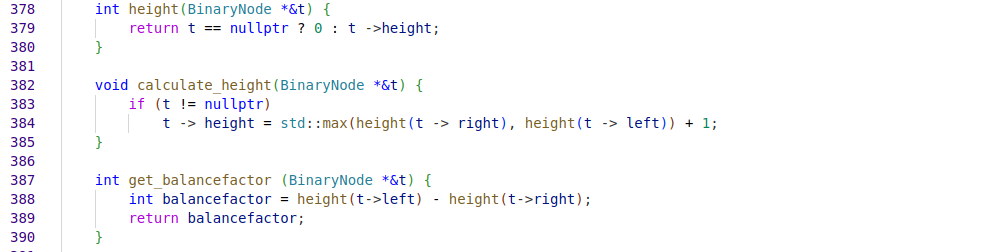
\includegraphics[width=0.7\textwidth]{fig1} %插入图片,[]中设置图片大小,{}中是图片文件名
		\caption{function about height} %最终文档中希望显示的图片标题
	\end{figure}
	
	随后我们设计VAL更改树结构的函数。右旋转为例进行说明。首先右旋转一次即需要创建一个新的结构体指针指向当前结点的左节点,我们称其为新节点。随后我们需要把将新节点的新右子节点连接将当前节点上,所以我们首先要将曾经的右子节点连接到当前节点的左节点上以保证树结构的完整性。进行完这两步操作之后,可以对节点高度进行一次迭代,随后将父节点指向当前节点的指针修改为指向新节点的指针,完成一次右旋转。
	
	左旋转与右旋转逻辑类似,只是中间左右节点相反。而其余两种情况则是需要考虑子节点的VAL判据。选择决定是否需要再进行左(右)旋转前先对右(左)子节点先进行一次右(左)旋转。
	

	
	\begin{figure}[H] %H为当前位置,!htb为忽略美学标准,htbp为浮动图形
		\centering %图片居中
		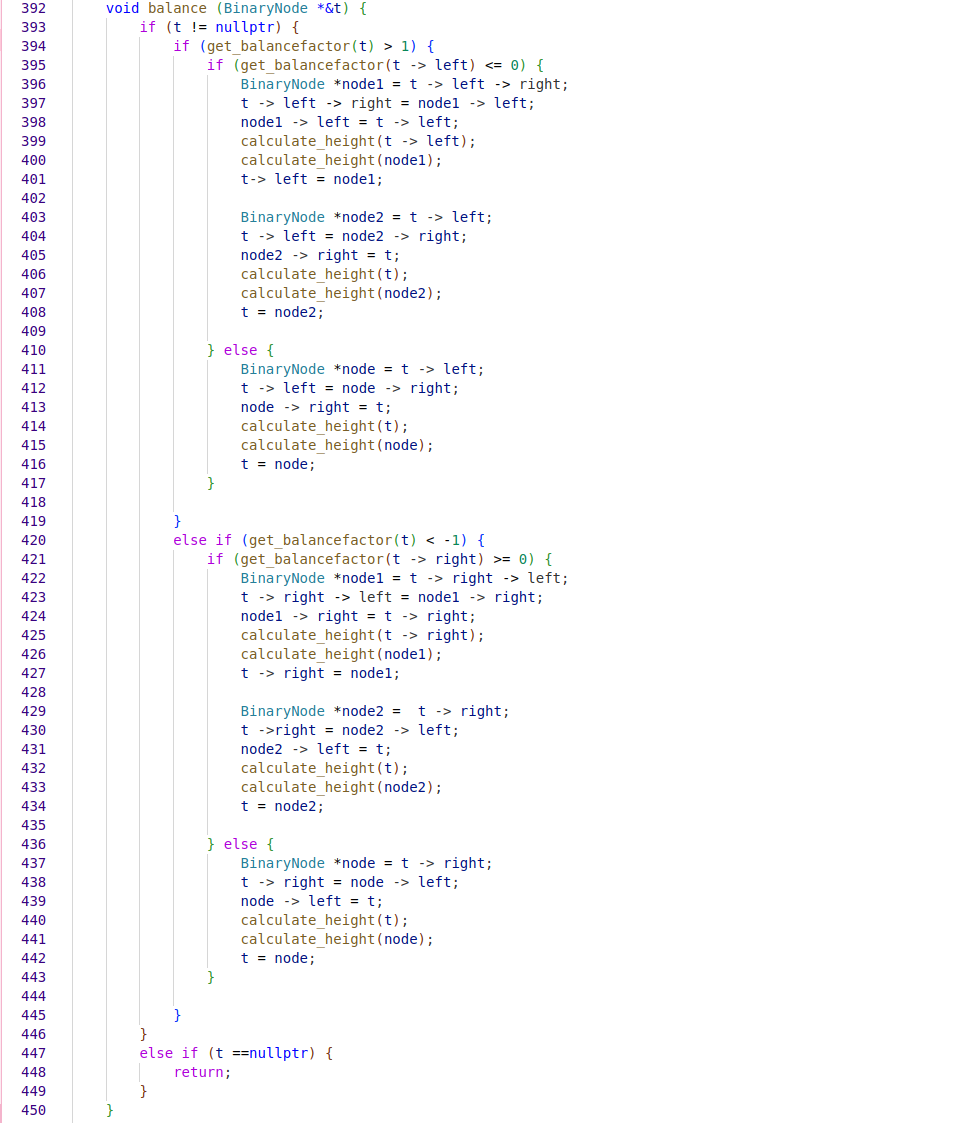
\includegraphics[width=0.7\textwidth]{fig2} %插入图片,[]中设置图片大小,{}中是图片文件名
		\caption{VAL\_balance} %最终文档中希望显示的图片标题
	\end{figure}
	
	
	
	最后是对remove函数的修改,只需要在remove节点之后调用上述函数即可。
	
	\begin{figure}[H] %H为当前位置,!htb为忽略美学标准,htbp为浮动图形
		\centering %图片居中
		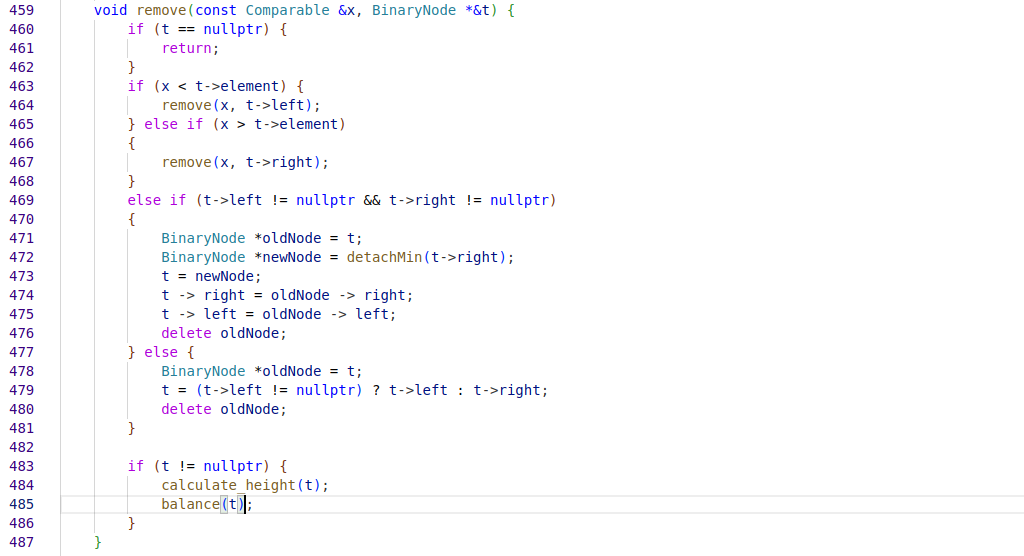
\includegraphics[width=0.7\textwidth]{fig3} %插入图片,[]中设置图片大小,{}中是图片文件名
		\caption{remove} %最终文档中希望显示的图片标题
	\end{figure}
	
	\section{测试的结果}
	
	测试结果一切正常。
	
	输出为: 
	
	\begin{figure}[H] %H为当前位置,!htb为忽略美学标准,htbp为浮动图形
		\centering %图片居中
		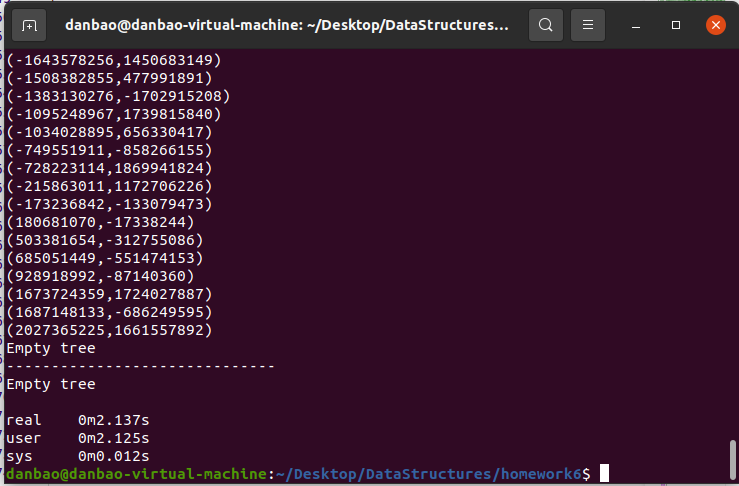
\includegraphics[width=0.7\textwidth]{fig4} %插入图片,[]中设置图片大小,{}中是图片文件名
		\caption{output} %最终文档中希望显示的图片标题
		\label{Fig.main2} %用于文内引用的标签
	\end{figure}
	
	
	\section{bug报告}
	
	一切正常。
	
	%%% Local Variables: 
	%%% mode: latex
	%%% TeX-master: t
	%%% End: 
\end{document}